\documentclass[12pt]{article}
\usepackage[spanish]{babel}

\usepackage{enumerate}
\usepackage{geometry}
	\geometry{margin= 2cm}
\usepackage{graphicx}
	\graphicspath{ {assets/} }
\usepackage{hyperref}
\usepackage{multicol}
\usepackage{amssymb}

%%%%%%%%%%%%%%%%%%%%%%%%%%%%%%%%%%
%%%%%%%%%%%%%%%%%%%%%%%%%%%%%   %%
%%        Datos Trabajo     %%  %%
%%%%%%%%%%%%%%%%%%%%%%%%%%%%%%%%%%
\newcommand{\titulo}[0]{Evidencia de aprendizaje: Problemáticas de su entorno}
\newcommand{\materia}[0]{Desarrollo Sustentable}
\newcommand{\grupo}[0]{BI-BDSU-2002-B1-012}
\newcommand{\unidad}[0]{Unidad 1}
%%%%%%%%%%%%%%%%%%%%%%%%%%%%%%%%%%
%%%%%%%%%%%%%%%%%%%%%%%%%%%%%%%%%%

\title{
	
\includegraphics{../../../assets/logo-unadm.png} \\
	\ \\\ \\Benjam\'in Rivera \\
	\bf{\titulo}\\\ \\}

\author{
	Universidad Abierta y a Distancia de México \\
	TSU en Biotecnolog\'ia \\
	\textit{Materia:} \materia \\
	\textit{Grupo:} \grupo \\
	\textit{Unidad:} \unidad \\
	\\
	\textit{Matricula:} ES202105994 }

\date{\textit{Fecha de entrega:} \today}


%%%%%%%%%%%%%%%%%%%%%%%%%%%%%
%%        Documento         %%
%%%%%%%%%%%%%%%%%%%%%%%%%%%%%%%
\begin{document}
\maketitle\newpage

\section*{Problem\'atica}
	\begin{center}\par\bf\huge Contaminaci\'on del aire por ladrilleras
	\end{center}
	
	\par Una actividad econ\'omica bastante popular en mi municipio, y tambi\'en en varios estados a lo largo de toda la rep\'ublica, es la producci\'on de ladrillo rojo. Dicha actividad requiere, en ciera parte de su producci\'on, utilizar grandes fuentes de calor para poder \textit{cocer} el ladrillo y que convertir el maleable adobe en ladrillos resistentes. 
	
\begin{figure}[h]
	\centering
	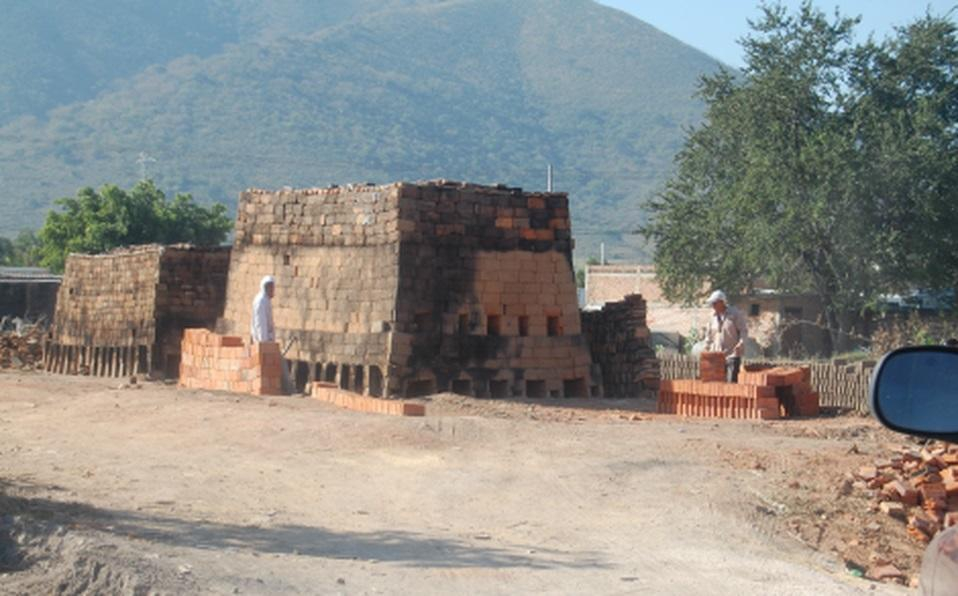
\includegraphics [width=0.5\textwidth] {quema_ladrillos.jpg}
	\caption{Horno de ladrillos en municipio de Guanajuato.}
\end{figure}

	\par En el paso antes descrito es donde se encuentra el problema, la mayor\'ia de los artesanos que se desempe\~nan en este oficio utilizan combustibles poco amigables con el ambiente, como llantas, plasticos, maleza y madera, y como lo hacen al aire libre, todas las particulas de estos materiales, que no se logran consumir en su totalidad, contaminan el aire circundante dejando las areas cercanas contaminadas.
	
\begin{figure}[h]
	\centering
	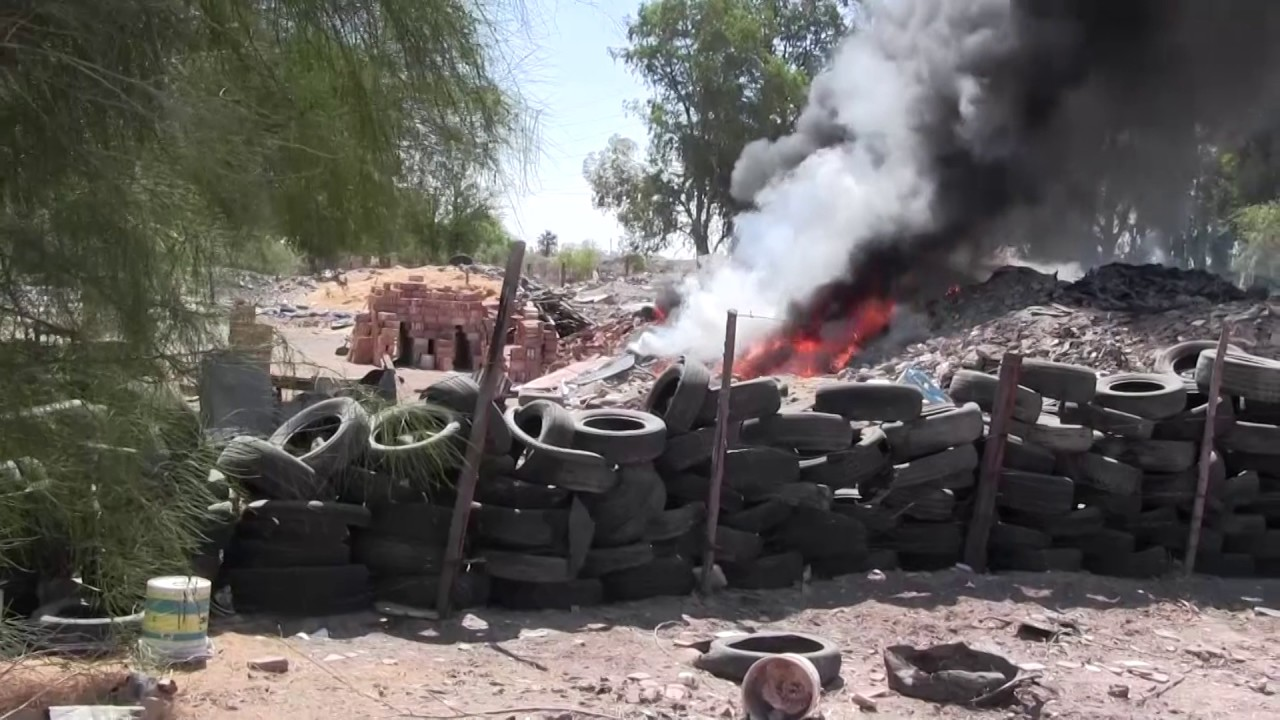
\includegraphics [width=0.5\textwidth] {fuego_ladrillos.jpg}
	\caption{Horno de ladrillos encendido y pilas de material utilizado en la combusti\'on.}
\end{figure}

	\par Esta contaminaci\'on del aire tiene distintas implicaciones, la m\'as evidente es que al final del proceso las areas circundantes quedan sumisas en una bruma, parecida a neblina, ocasionada por las part\'iculas suspsendidas en el aire, esto esta evidenciado en \cite{ladrillos-visual}. Estas mismas particulas pueden provocar diversas enfermedades a las personas que vivan cerca o incluso que transiten la zona, como exploraron en \cite{enfermedades}. E incluso esta situaci\'on llega a afectar un recurso tan preciado como el agua, evidenciado en \cite{agua}.

	\par Algunas de las razones que se han identificado como parte de este problema incluyen:
	\begin{quote}\begin{enumerate}
		\item Falta de conciencia por parte de los artesanos.
		\item Apat\'ia por los afectados.
		\item Apego a las tradiciones o desconocimiento de metodos m\'as eficientes por parte de los artesanos. \label{tradicion}
		\item Falta de apoyos gubernamentales para modernizaci\'on del proceso. \label{gobierno}
	\end{enumerate}\end{quote}
	
\begin{figure}[]
	\centering
	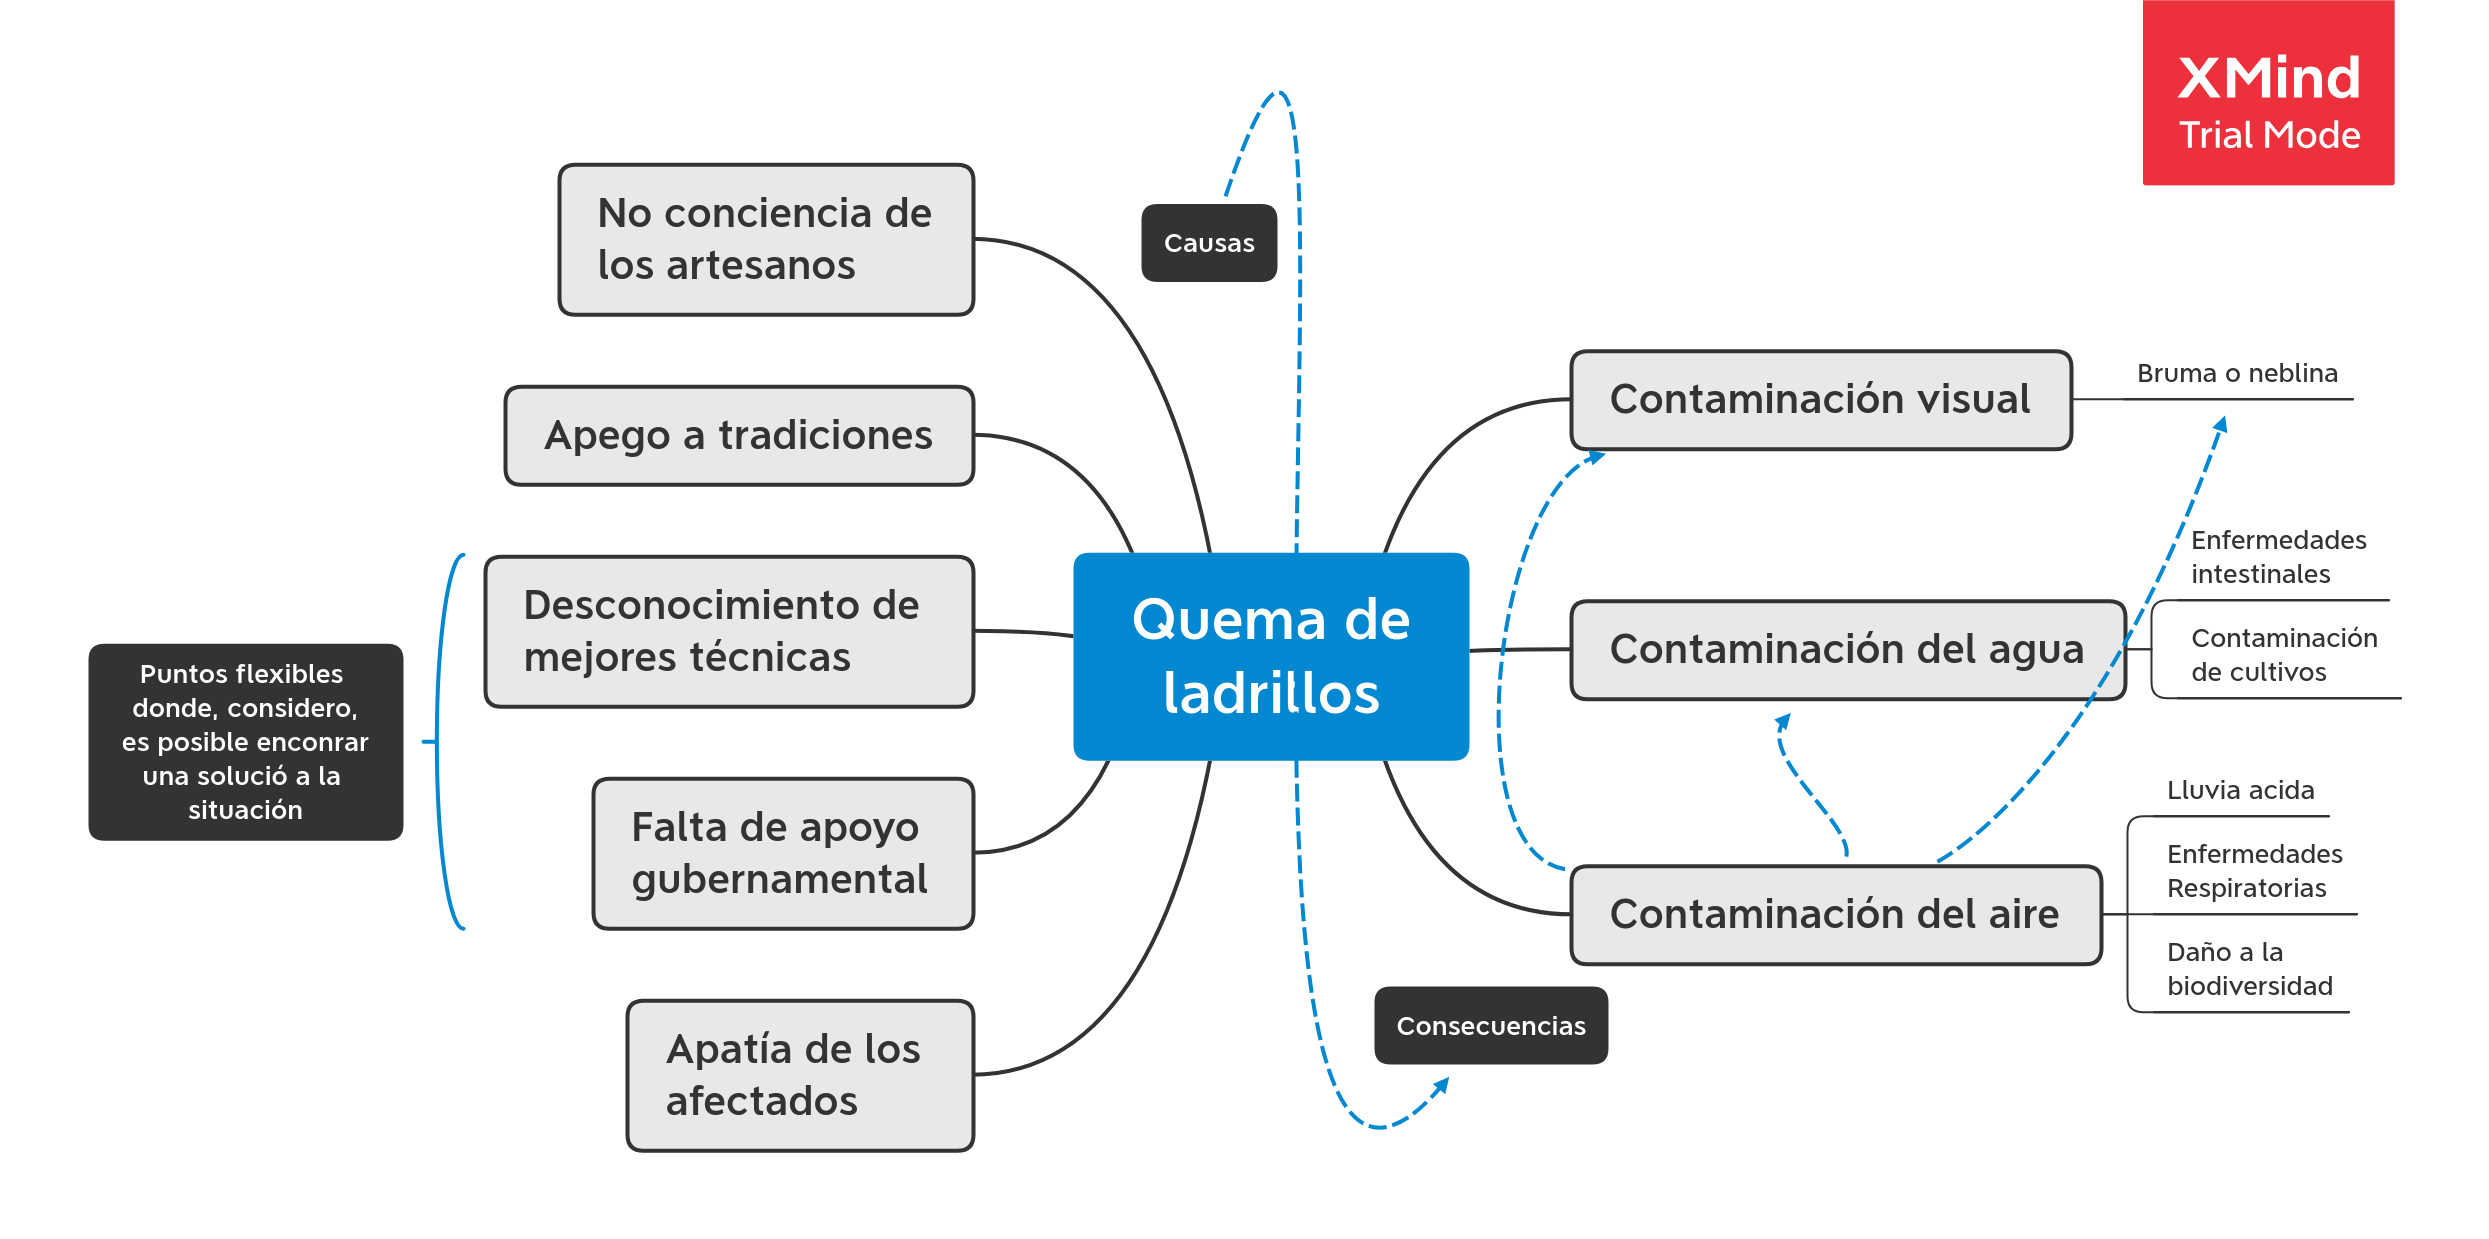
\includegraphics [width=\textwidth] {Mapa_ladrillos.png}
	\caption{\'Arbol de problemas horizontal de la \textit{quema de ladrillos}.}
\end{figure}
	
	\par Los dos primeros puntos son los m\'as complicados de solucionar, ya que requiere todo un cambio de cultura de una cantidad considerable de personas. Respecto al punto \ref{tradicion} creo que ser\'ia un interesante punto para explorar, aunque el detalle con los metodos m\'as modernos, y que menos afectan al ambiente, es que requieren una inversi\'on inicial alta, donde creo que, si se solucionea el punto \ref{gobierno}, esta un plan de acci\'on que puede tratar de solucionar esta situaci\'on.
	




%%%%%%%%%%%%%%%%%%%%%%%%%%%%%%%%
%%         Bibliografia        %%
%%%%%%%%%%%%%%%%%%%%%%%%%%%%%%%%%%

\begin{thebibliography}{X}
	\bibitem{ladrillos-visual} Edición. (2020). {\it Supera contaminación de ladrillos a administraciones}. 15 de Julio de 2020, de Perdiodico Correo Sitio web: \url{https://periodicocorreo.com.mx/supera-contaminacion-de-ladrillos-a-administraciones/}
	\bibitem{enfermedades} Gallegos, A., Lang, B., Fernandez, M. \& Lujan, M.. (2006). Contaminaci\'on atmosf\'erica por la fabricaci\'on de ladrillos y sus posibles efectos sobre la salud de los ni\~nos de zonas aledañas. 17 de Julio de 2020, de Universidad Cat\'olica Boliviana Sitio web: \url{http://www.scielo.org.bo/pdf/ran/v3n2/v3n2_a04.pdf}
	\bibitem{agua} Romo, M., Cordova, G \& Cervera, L.. (2004). Estudio urbano-ambiental de lasladrilleras en el municipio de Juáre. 17 de Julio de 2020, de El Colegio de la Frontera Norte Sitio web: \url{http://www.scielo.org.mx/pdf/estfro/v5n9/v5n9a1.pdf}

\end{thebibliography}
\end{document}